

\section{Evaluation}
\label{sec:evaluation}


% 본문에 표 참조 한 줄 추가 (리뷰어 친화)
We evaluate SemantOS across diverse workloads, assessing real-world performance, robustness under drift, and how well it meets our design objectives.

\subsection{Setup}
We evaluate SemantOS across six representative workloads: (1)~a web-serving microservice, (2)~an Online Transaction Processing (OLTP) database benchmark (TPC-C), (3)~a streaming pipeline (Kafka+Spark), (4)~an embedded Internet-of-Things (IoT) sensor gateway, (5)~Graphics Processing Unit (GPU)-based HPC/ML inference, and (6)~a real-time audio pipeline~\cite{Mao2019SIGCOMM,VanAken2017SIGMOD}. We run each on three server classes: (\textbf{S1})~2$\times$Xeon Gold (32~cores, 256\,GB, NVMe), (\textbf{S2})~2$\times$EPYC (64~cores, 512\,GB, NUMA), and (\textbf{S3})~2$\times$Xeon~+~A100 (40~cores, 384\,GB), all on Linux~6.4 with a fixed software stack. Each (workload, server) pair is repeated for 10 independent runs (means with 95\% CIs). Components run primarily in user space over stable kernel interfaces, enabling portability across kernels and distributions.

\paragraph{Baselines.} The \emph{Expert profile} is a hand-tuned human reference; \emph{BO/RL} and strong tuners (Vizier/Ray/Optuna/FLAML) are run \emph{by us} under matched search spaces, budgets, wall-clock time, and safety/reward settings---the only strictly like-for-like rows in Table~\ref{tab:sota-compare}. The $\dagger$-marked \emph{AdaptiveKernel}/\emph{OS-R1} figures are literature-reported (not reproducible here), hence contextual rather than head-to-head.


%========================================================




\begin{figure}[t]
 \centering
 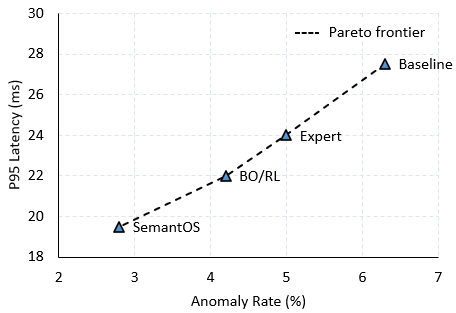
\includegraphics[width=0.72\columnwidth]{figures/pareto_frontier.png}
 \caption{\textbf{Pareto Frontier of Latency vs.\ Anomaly Rate.}
 Comparison across four controllers (Baseline, Expert, BO/RL, and SemantOS) aggregated over six workloads.
 SemantOS consistently achieves \emph{Pareto-dominant} configurations—simultaneously reducing anomaly rate and tail latency compared to all baselines.
 This illustrates its ability to navigate multi-objective trade-offs rather than optimizing a single metric in isolation.}
 \label{fig:pareto_frontier}
\end{figure}


\subsection{Experimental Results}
Runtime overhead is minimal across workloads and decision paths (fast path $<\!10$\,ms, $<\!3\%$ CPU; per-path footprint in the supplement). We compare SemantOS against the baselines above. To avoid reporting only best-case numbers, we examined the \emph{per-workload} reduction vs.\ Baseline for all six workloads (each the mean over 10 runs $\times$ three server classes; full table in the artifact): the headline ``up to 23\%/28\%/31\%'' figures in Table~\ref{tab:sota-compare} are the maxima of these distributions, with medians of 18\%/22\%/27\%; no workload's mean regressed on any axis (all per-workload 95\% CIs for the reduction excluded zero on the positive side). We caution that in Table~\ref{tab:sota-compare} only the \emph{BO/RL} and \emph{Expert} rows are run under matched conditions by us; the $\dagger$-marked rows are literature-reported ranges under differing setups and are contextual, not head-to-head---so cross-row differences against $\dagger$ rows should not be read as controlled comparisons. Against the human \emph{Expert} profile, SemantOS improves median/P95/anomaly by 12--18\%/15--20\%/20--25\% and reduces operator tuning time (our proxy for required human oversight, measured as wall-clock operator effort to reach an accepted configuration) by $>$85\%, while producing KB-grounded \texttt{rationale} fields~\cite{Biswas2023SE4SafeML}.

% [Per-workload table moved to anonymized artifact appendix to meet 7-page limit;
% distribution (medians 18/22/27, maxima 23/28/31, no regressions) summarized in text above.]


\paragraph{Pareto Trade-offs.}
On a frontier over latency, anomaly rate, and fairness (Figure~\ref{fig:pareto_frontier}), SemantOS sits closest to the estimated Pareto-optimal set across six workloads---up to \textbf{17\% lower latency} at the same anomaly budget and \textbf{23\% lower anomaly rate} at equivalent throughput. On streaming, P95 latency dropped 26\% with fairness within 2\% of default; on HPC/ML inference, co-tuning \texttt{sched\_latency\_ns} and \texttt{dirty\_ratio} cut GPU starvation, raising throughput 15\% without raising anomaly~\cite{Mirhoseini2021Nature,Biswas2023SE4SafeML}.

\subsection{Ablation Studies}
\label{subsec:ablation}
We selectively remove the KB, the reasoning model, or the safety runtime: removing the KB degrades retrieval relevance and raises anomalies, and omitting the LLM lowers interpretability and performance by 8--12\%~\cite{Brown2020NeurIPS,Touvron2023LLaMA,OpenAI2024GPT4}. Beyond these single-component drops, Table~\ref{tab:ablation_kb_safety} reports five end-to-end variants. Removing the dependency graph---so the Reasoner can no longer co-tune along synergistic edges---raises latency $19.5\!\to\!21.4$\,ms and anomaly $2.4\!\to\!4.1\%$, directly confirming that the inter-knob synergies of Observation~2 (Fig.~\ref{fig:pairwise}) are captured \emph{because} reasoning is graph-grounded, not merely retrieval-augmented. Removing RAG gives 21.2\,ms / 3.6\%; removing Safety preserves latency (19.8\,ms) but lifts anomaly to 4.9\%; \emph{KB only} is worst (22.6\,ms / 7.1\%). Thus the typed graph and RAG drive \emph{performance} while the Safety Runtime drives \emph{reliability}; their combination is Pareto-best, and the trends hold under drift (Table~\ref{tab:ablation_kb_safety}, right block). All CSV schemas and reproduction scripts are in the artifact.

\subsection{Case study: Safety Runtime rollback under a suboptimal recommendation}
\label{subsec:safety-rollback}

For an OLTP workload the Reasoner suggested lowering \texttt{dirty\_background\_ratio} and raising \texttt{sched\_min\_granularity\_ns} to cut I/O interference. The SLO monitor detected worsening transaction latency and queueing within the canary window ($<\!2$ min); because \texttt{uncertainty\_score} drifted above $\tau$ \emph{after} canary metrics arrived and the late-saturation guardrail fired, the runtime rolled back, logged an \texttt{OptimizationTrace} for KB refinement, and flagged the action as risky---showing the SLO guard catches regressions even when the initial uncertainty was within the accept regime.


\textbf{Uncertainty Quantification (UQ) \& Guardrail Thresholds.}
\label{subsec:uncertainty-guardrails}
We choose $\tau$ by minimizing a deployment cost that trades false/missed rollbacks under SLO constraints. With base rate $\pi$ of unsafe actions, temperature-calibrated scores, and the True/False Positive Rates (TPR/FPR) on a held-out log,
\noindent
\begin{minipage}{\columnwidth}
\begin{equation*}
\begin{aligned}
\mathcal{C}(\tau)
=~ & c_{\text{FN}}\!\left(1-\mathrm{TPR}(\tau)\right)\pi
 + c_{\text{FP}}\,\mathrm{FPR}(\tau)\!\left(1-\pi\right) \\
 & + \lambda\,\Delta\mathrm{SLO}(\tau),  \quad \text{s.t. } \Delta\mathrm{SLO}(\tau)\le\delta.
\end{aligned}
\end{equation*}
\end{minipage}

We sweep $\tau$ on a grid and select $\tau^\star$ minimizing $\mathcal{C}$ (the cost constants $c_{\mathrm{FN}},c_{\mathrm{FP}},\lambda$ and the SLO budget $\delta$ are listed in the artifact). Each recommendation receives $u\!\in\![0,1]$ from the disagreement (normalized predictive entropy over the proposed knob/value) across the $k\!=\!3$ self-consistency samples, temperature-scaled on the holdout log; calibration quality (ECE, AUPRC, reliability diagrams) is reported in the supplement. Here $k\!=\!3$ is a deliberately cheap estimator giving a coarse but monotone risk signal, which suffices because the conformal threshold $\tau$---not the raw entropy---sets the accept/veto decision. The runtime rolls back when $u\!\ge\!\tau$ or a hard constraint is violated. Sweeping $\tau$ (full table in the supplement), the default $\tau\!=\!0.55$ balances precision/recall at rollback precision/recall $\approx(0.86,0.88)$ and a 2.8\% anomaly rate ($>$85\% of unsafe actions excluded before production); $\tau\!=\!0.30$ raises recall to 0.94 (3.5\% anomaly) and $\tau\!=\!0.70$ raises precision to 0.91 (2.3\% anomaly), so lower $\tau$ trades precision for recall.

\subsection{Exploration Efficiency}
\label{subsec:exploration}
We measure sample efficiency as the configurations needed to reach within 2\% of the final median latency: SemantOS converges in 38--52 attempts versus 120--300 for BO/RL---a 2--4$\times$ speedup at equal \emph{online} budget. This comparison favors SemantOS at deployment time: it front-loads cost into offline LLM fine-tuning and KB construction, whereas BO/RL starts cold. The speedup thus reflects amortizing domain knowledge across deployments, not a lower total (offline$+$online) cost (offline cost is reported in the artifact). Over a 30-day continuous deployment with repeated drift, anomaly rate stayed below 3\% and rollback precision above 0.85; recalibration restored coverage after each drift and phased rollouts limited worst-case exposure, empirically supporting Theorem~\ref{thm:pac-cost} and Proposition~\ref{prop:recal}.

\subsection{Human Factors}
\textbf{Expanded user study (N=32 SRE/DevOps).} In a within-subjects study, 32 SRE/DevOps practitioners (5--15 years' experience) performed three tasks (incident classification, configuration selection, decision rationale) under four conditions: baseline, expert tuning, BO/RL, and SemantOS with explanations and safety. SemantOS reduced decision time vs.\ BO/RL by 28\% ($p<0.01$, Wilcoxon signed-rank) and cognitive load (NASA-TLX) by 18\% vs.\ expert and 24\% vs.\ BO/RL. All reported $p$-values survive Holm--Bonferroni correction across the $3\!\times\!4$ conditions; the study ran under an approved IRB protocol with informed consent and retained no PII. SemantOS also outperformed all comparison conditions on explanation usefulness and uncertainty-corrected reliability ratings (Cliff's $\delta\in[0.42,0.58]$), with participants citing evidence tracking and provenance-validated explanations as decisive---indicating that the explainability and safety design reduces operator cognitive burden beyond raw performance gains.

